\begin{figure}
    \begin{center}
        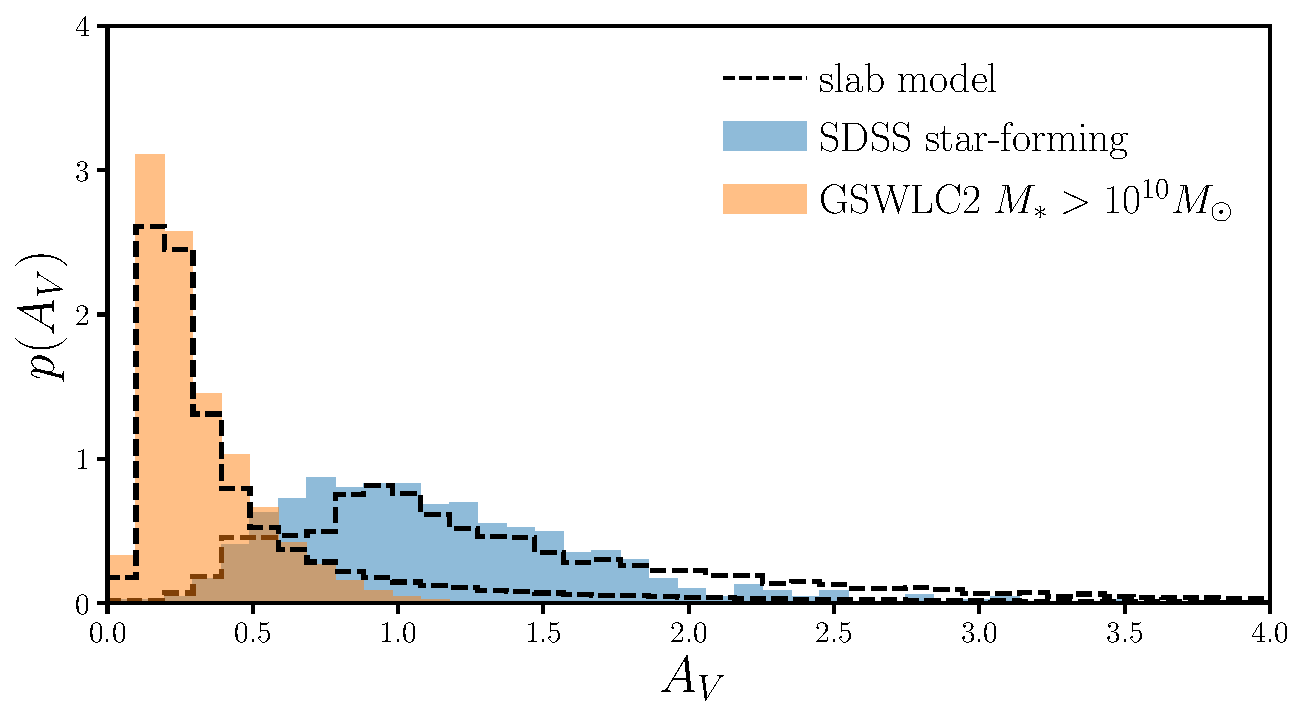
\includegraphics[width=0.66\textwidth]{figs/slab_model.pdf} 
        \caption{\label{fig:av_dist}
        The $A_V$ distributions, $p(A_V)$, generated from the slab model (Eq.~\ref{eq:slab};
        black dash) compared to $p(A_V)$ of star-forming galaxies our SDSS
        sample (blue; Section~\ref{sec:obs}) and of $M_* > 10^{10}M_\odot$
        star-forming and quiescent galaxies in the GSWLC2 sample (orange). 
        The $A_V$ values for both observations are derived using SED
        fitting but with different bands and methodologies~\citep{brinchmann2004, salim2018}. 
        For the slab model, we generate $A_V$ values for each galaxy
        in the SDSS and GSWLC2 samples using Eq.~\ref{eq:slab} with its
        measured $M_*$ and $\ssfr$ and randomly sampled $i$. 
        Despite the significant differences between the $p(A_V)$ of SDSS and
        GSWLC2, the slab model is able to generate $p(A_V)$ in good agreement
        with both observations using parameter values within the
        Table~\ref{tab:free_param} prior range. 
        Therefore, the slab model provides a sufficiently flexible prescription
        for our \eda.
        }
    \end{center}
\end{figure}


\section{The Slab Model Based EDA}  \label{sec:slab} 
In our \eda~prescription, we use the slab model to determine $A_V$, the
amplitude of attenuation, as a function of a randomly sampled inclination,
$i$, and $\tau_V$ (see Eq.~\ref{eq:slab} in Section~\ref{sec:dem}).
The slab model is based on the assumption that dust in galaxies have
slab-like geometry and are illuminated by the stellar radiation
source~\citep{somerville1999}. 
For a given $\tau_V$, the attenuation depends solely on the orientation of the galaxy. 
While this simplification reproduces the correlation between $A_V$ and $i$
found in observed star-forming galaxies~\citep[\eg][]{conroy2010, wild2011,
battisti2017, salim2020}, it ignores the detailed star-to-dust geometry that
impacts the attenuation curve. 
It also does not provide a physically-motivated prescription for quiescent
galaxies, which typically have elliptical morphologies.
Despite its limitations, the slab model provides a robust empirical
prescription that allows us to produce realistic distributions of $A_V$. 

In Figure~\ref{fig:av_dist}, we compare the $A_V$ distributions, $p(A_V)$,
of star-forming galaxies in SDSS (blue) and galaxies in the
\cite{salim2018} GSWLC2 sample (orange) to $p(A_V)$ generated from the
slab model (black dashed). 
The $A_V$ values of the SDSS are derived using SED fitting from the
\cite{brinchmann2004} MPA-JHU catalog.
The GSWLC2 $A_V$ values are also derived from SED fitting UV and optical
photometry from GALEX and SDSS observations as well as mid-IR photometry from WISE. 
The GSWLC2 $p(A_V)$ includes all galaxies, including quiescent ones, above
$M_* > 10^{10}M_\odot$. 
We generate two $p(A_V)$ with the slab model for the SDSS and GSWLC2
samples separately.
For each SDSS/GSWLC2 galaxy, we determine $A_V$ by uniformly sampling 
$\cos i$ from 0 to 1 and derive $\tau_V$ (Eq.~\ref{eq:tauv}) with the
galaxy's measured $M_*$ and $\ssfr$. 
We pick $\mtaum, \mtaus, c_\tau$ values within the prior range
(Table~\ref{tab:free_param}) by hand to roughly reproduce the SDSS and GSWLC2 $p(A_V)$
distributions. 

Galaxies in SDSS and GSWLC2 have substantially different $p(A_V)$. 
While the galaxy populations only partially overlap, this difference is 
{\em mostly} due to inconsistencies in the $A_V$ measurements of MPA-JHU and GSWLC2 --- even
for the same galaxy.
%In fact for the ${\sim}8000$ galaxies that are in both samples, the $A_V$ distributions appear similar to those of the corresponding complete samples.}
This difference in $p(A_V)$ illustrates the challenges in directly measuring
dust attenuation. 
Despite the dramatic differences between the two, the slab model can
produce $p(A_V)$ in good agreement with both observed distributions. 
We therefore conclude that the slab model provides a sufficiently flexible
prescription to sample a realistic distribution of $A_V$. 

\begin{figure}
\begin{center}
    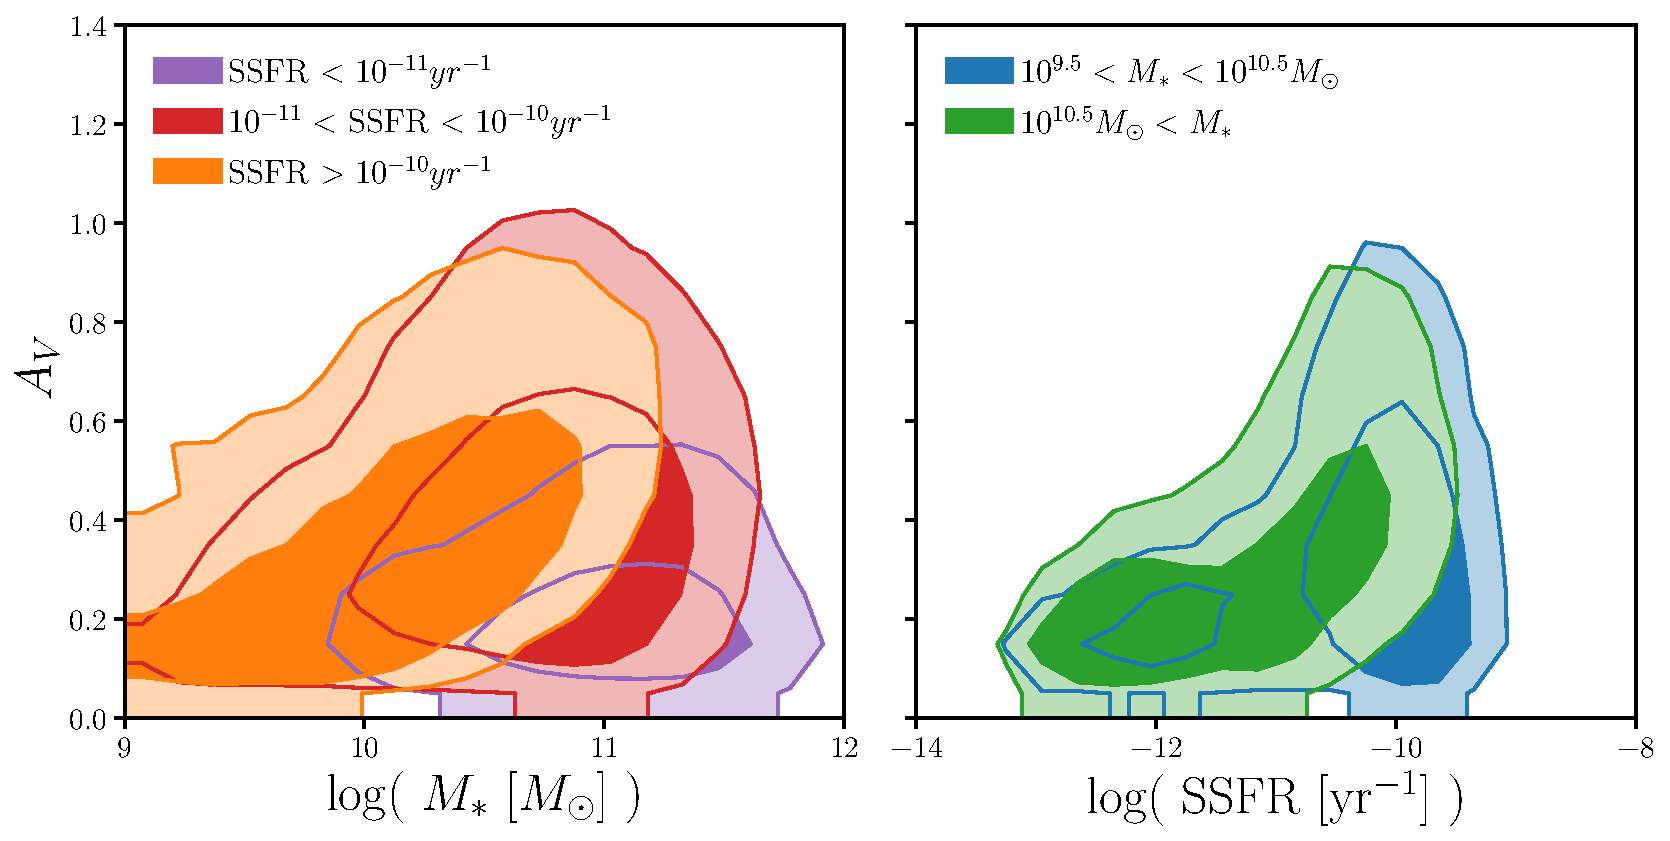
\includegraphics[width=0.8\textwidth]{figs/gswlc_dep.pdf}
    \caption{\label{fig:dep}
    Dependence of $A_V$ on $M_*$ (left) and $\ssfr$ (right) for the
    \cite{salim2018} GSWLC2 sample.
    In the left panel, we divide the GSWLC2 sample into bins of $\ssfr$: 
    $\ssfr < 10^{-11}yr^{-1}$ (purple), 
    $10^{-11} < \ssfr < 10^{-10}yr^{-1}$ (red),
    and  $10^{-10} < \ssfr$ (orange). 
    In each of the $\ssfr$ bins, we find significant $M_*$ dependence. 
    In the right panel, we divide the sample into bins of $M_*$:  
    $10^{9.5} < M_* < 10^{10.5}M_\odot$ (blue) and $10^{10.5} M_\odot < M_*$ (green).
    In the $M_* > 10^{10.5}M_\odot$ bin, which roughly corresponds to our
    SDSS sample, we find significant $\ssfr$ dependence.
    The $M_*$ and $\ssfr$ dependence in $A_V$ we find in GSWLC2 is
    consistent with previous works and provides further motivation for our
    \eda~prescription.
    }
\end{center}
\end{figure}

In addition to the slab model, in the \eda, we also use a linear
dependence on $M_*$ and $\ssfr$ in the $V$ band optical depth,
$\tau_V$ (see Eq.~\ref{eq:tauv}).
This parameterization is motivated by observations that find significant
correlation between $A_V$ and $M_*$ and $\ssfr$~\citep[\eg~][]{garn2010, battisti2016, salim2020}. 
We take a closer look at this correlation using the GWSLC2 sample in
Figure~\ref{fig:dep}.
We present the dependence of $A_V$ on $M_*$ (left panel) and $\ssfr$ (right
panel). 
In the left panel, we divide the GSWLC2 galaxies by $\ssfr$: 
$\ssfr < 10^{-11}yr^{-1}$ (purple), $10^{-11} < \ssfr < 10^{-10}yr^{-1}$
(red), and  $10^{-10} < \ssfr$ (orange). 
For each of the $\ssfr$ bins, we find significant $M_*$ dependence in
$A_V$: more massive galaxies have higher $A_V$.
In the right panel, we divide the galaxies by $M_*$: 
$10^{9.5} < M_* < 10^{10.5}M_\odot$ (blue) and $10^{10.5} M_\odot < M_*$
(green).
In both $M_*$ bins, galaxies with higher $\ssfr$ have higher $A_V$. 
The dependence is stronger stronger for galaxies with $M_* > 10^{10.5}M_\odot$, 
which roughly corresponds $M_*$ limit of our forward model (see
Figure~\ref{fig:avmsfr}). 
Overall, the $M_*$ and $\ssfr$ dependence we find in $A_V$ from the GSWLC2 sample is
consistent with previous observations and further motivates our
\eda~prescription.

\begin{figure}
\begin{center}
    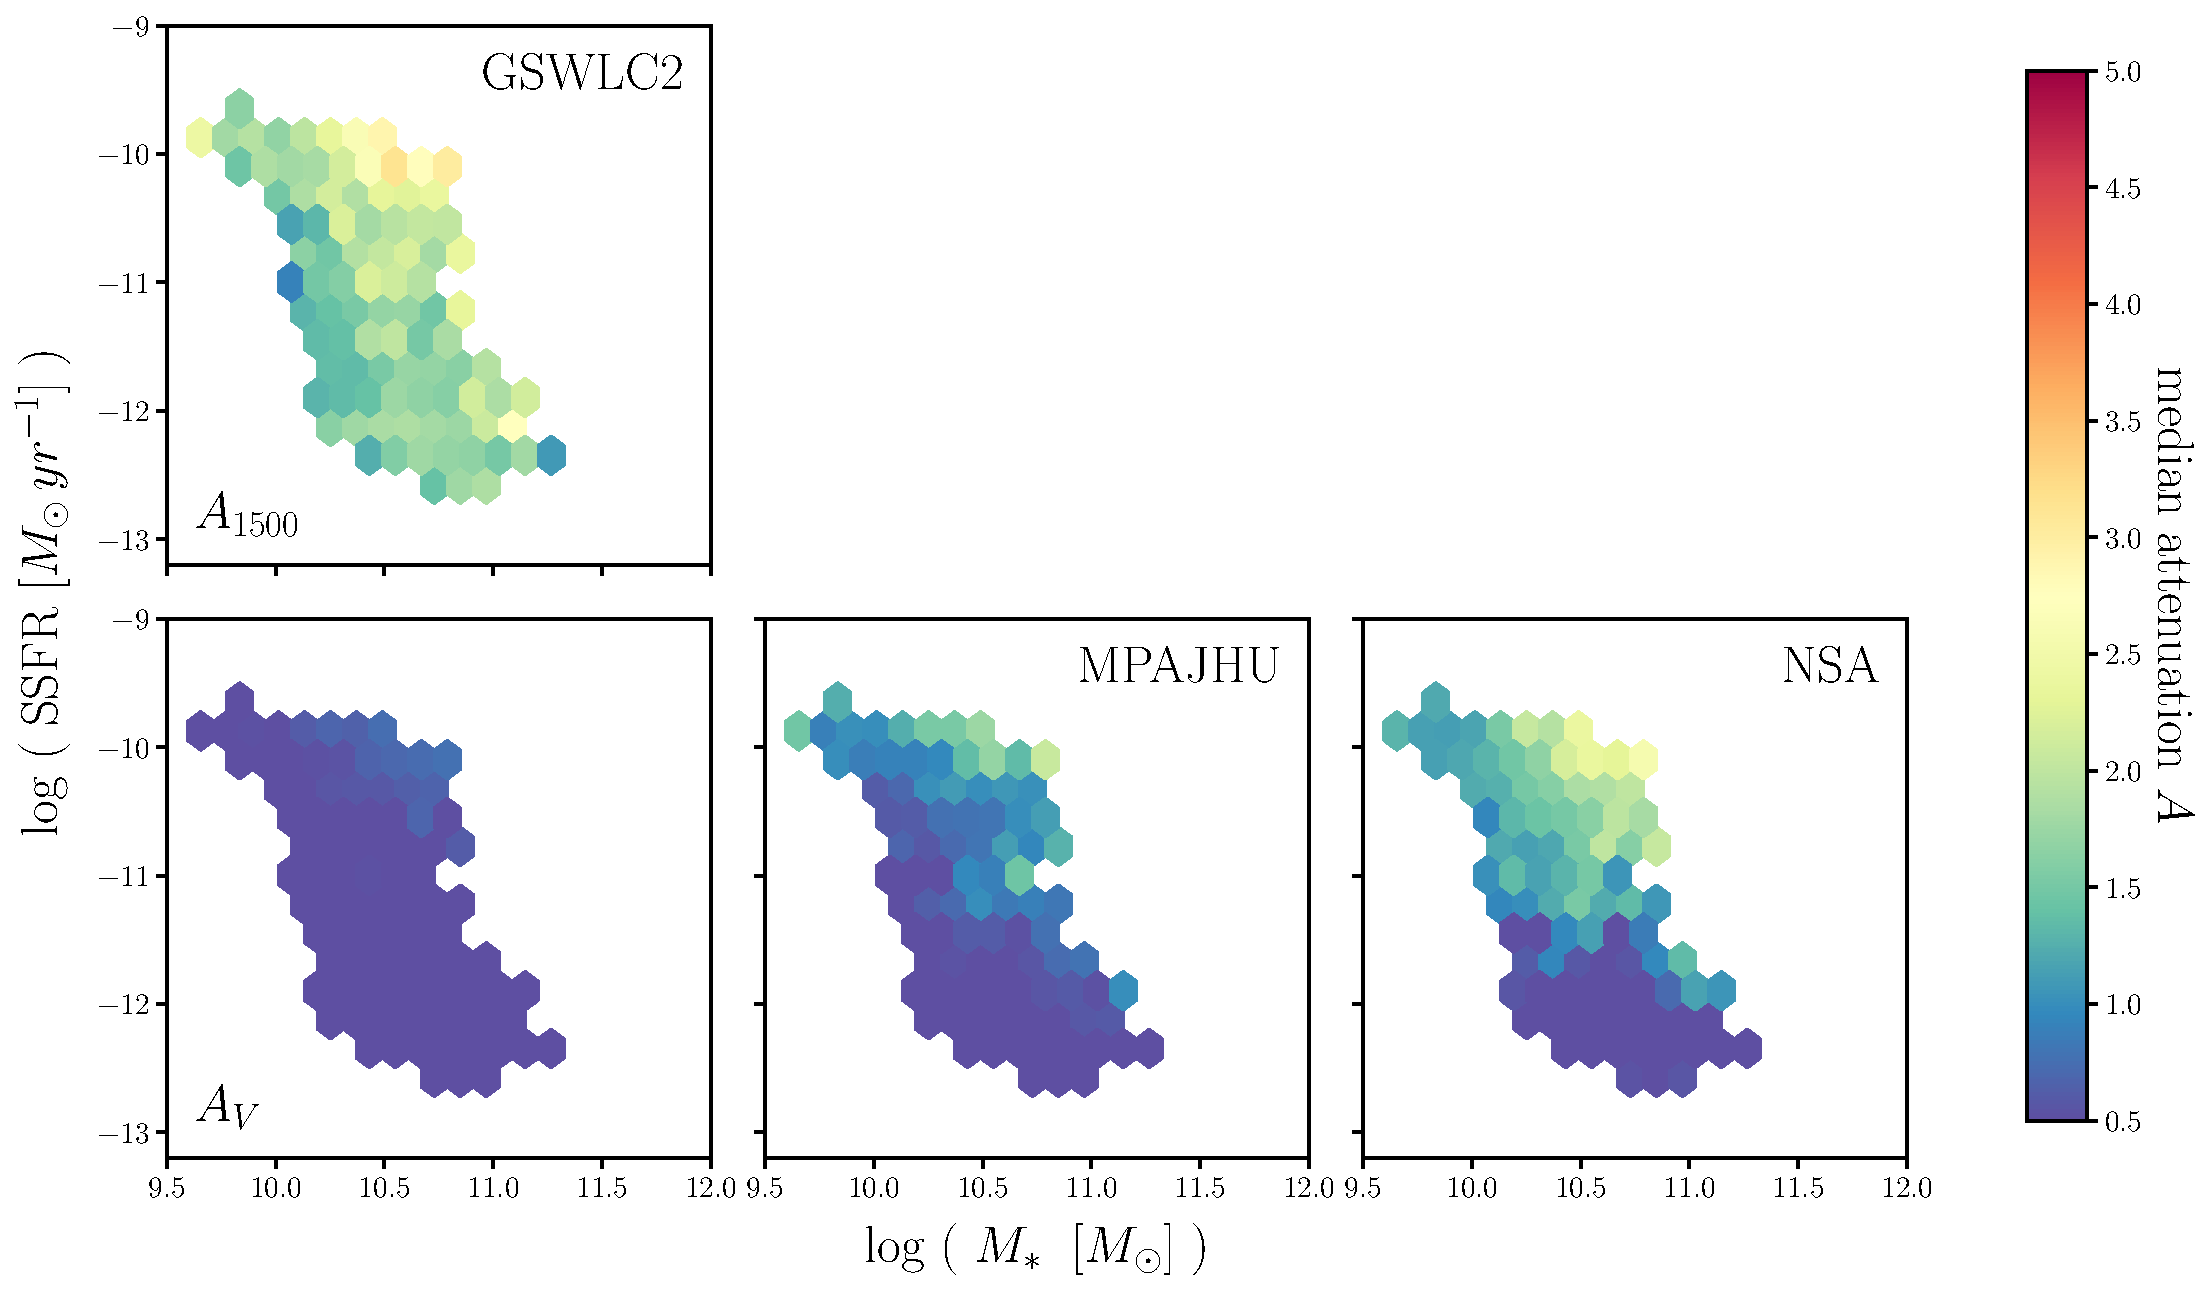
\includegraphics[width=\textwidth]{figs/av_mssfr_obs.pdf}
    \caption{\label{fig:av_obs}
    $M_*$ and $\ssfr$ dependence of dust attenuation at $1500 \AA$
    ($A_{1500}$; top) and at $5500\AA$ ($A_{V}$; bottom) of SDSS galaxies. 
    The sample includes 2361 galaxies that pass our selection cut
    (Section~\ref{sec:obs}) and are also part of the GSWLC2 and MPA-JHU
    samples. 
    In the left panels, we use $A_{1500}$ and $A_V$ from GSWLC2.
    In the center panel, we use $A_V$ from MPA-JHU. 
    In the right panel, we use $A_V$ from the NSA. 
    The $M_*$ and $\ssfr$ in each panel are from the respective samples. 
    Same as Figure~\ref{fig:avmsfr}, the colormap in each hexbin represents the
    median attenuation for all galaxies in the bin (color bar).
    We only include bins with more than 5 galaxies.
    The bottom panels illustrate that $A_V$ measurements from GSWLC2, MPA-JHU,
    and NSA differ {\em significantly} even for the same galaxies.
    We, therefore, do not directly compare our \eda~predictions to observations. 
    }
\end{center}
\end{figure}

In Figure~\ref{fig:av_obs}, we present the $M_*$ and $\ssfr$ dependence of dust
attenuation in SDSS galaxies, which contains 2361 galaxies that pass our
selection cut and are also in the GSWLC2 and MPA-JHU samples.
In the top panel, we present $A_{1500}$ from GSWLC2 as a function of $M_*$ and
$\ssfr$.
In the bottom panels, we present $A_V$ from GSWLC2 (left), MPA-JHU (center),
and NSA (right).
The NSA $A_V$ measurements are derived assuming intrinsic Balmer decrement of
2.85, $R_V=3.1$ and \cite{odonnell1994} extinction. 
The colormap in each hexbin represents the median attenuation for galaxies in
the bin, same  as in Figure~\ref{fig:avmsfr}. 
Bins with less than 5 galaxies are omitted. 
For each observational sample (column), we use $M_*$ and $\ssfr$ from the
respective samples for consistency.
We find the same $M_*$ and $\ssfr$ dependence of $A_V$ as Figure~\ref{fig:dep}
even after our selection cut (bottom left). 
The bottom panels highlight that evven for the same galaxies, $A_V$ from
GSWLC2, MPA-JHU, and NSA have significant differently amplitudes. 
$M_*$ and $\ssfr$ are also significantly different across the samples.
Since observations have large discrepancies among dust attenuation measurements
and a detailed comparison is beyond the scope of this work, we refrain from
comparing our \eda~predicted dust attenuation (Section~\ref{sec:results}) to
observations.
